\subsection{Reflecting Boundaries with Vision}

\begin{frame}
	\frametitle{3) Reflecting Boundaries}
	\textbf{Trajectory.} Example.
	\begin{itemize}
	    \item $\rho = 400, v = 0.03, R = 0.03, D_{\text{rot}} = 0.01, \Delta t = 1.0, N_{\text{sim}} = 1500, N_{\text{eq}} = 1000$
	    \item Representative trajectory is shown
	    \item Large fluctuations (collisions with boundary)
	\end{itemize}
	\begin{figure}[H]
  		\includegraphics[width=\textwidth]{images/chapter3/flocks_N_20_L_1.000000_v_0.030000_R_0.010000_D_0.010000.png} 
  		%\caption*{Cantillano C., Grundpraktikum 2: Halbleiterbauelemente. Internal Proceedings. University of Innsbruck , 2021.}
	\end{figure}
\end{frame}

\begin{frame}
	\frametitle{3) Reflecting Boundaries}
	\textbf{Trajectory.} Interesting Collisions.
	\begin{itemize}
	    \item $\rho = 400, v = 0.03,  R = 0.03, D_{\text{rot}} = 0.01, \Delta t = 1.0, N_{\text{sim}} = 1500, N_{\text{eq}} = 1000$
	    \item Two incoming flocks $\rightarrow$ one outgoing flock 
	\end{itemize}
	\begin{figure}[H]
  		\includegraphics[width=\textwidth]{images/chapter3/collision_N_20_L_1.000000_v_0.030000_R_0.030000_D_0.010000.png} 
  		%\caption*{Cantillano C., Grundpraktikum 2: Halbleiterbauelemente. Internal Proceedings. University of Innsbruck , 2021.}
	\end{figure}
\end{frame}

\begin{frame}
	\frametitle{3) Reflecting Boundaries}
	\textbf{Configurations.} $R$-dependence.
	\begin{itemize}
	    \item $\rho = 400, v = 0.03, D_{\text{rot}} = 0.01, \Delta t = 1.0, N_{\text{sim}} = 1500, N_{\text{eq}} = 1000$
	    \item Bigger $R\Rightarrow$ bigger flocks 
	    \item Flocking stronger compared to periodic boundaries
	\end{itemize}
	\begin{figure}[H]
  		\includegraphics[width=\textwidth]{images/chapter3/N_20_L_1.000000_v_0.030000_R_D_0.010000_rbc.png} 
  		%\caption*{Cantillano C., Grundpraktikum 2: Halbleiterbauelemente. Internal Proceedings. University of Innsbruck , 2021.}
	\end{figure}
\end{frame}

\begin{frame}
	\frametitle{3) Reflecting Boundaries}
	\textbf{Phase transitions.} 2D Levels in parameter space.
	\begin{itemize}
	    \item $R$ against $\sqrt{2D_{\text{rot}}\Delta t}$
	\end{itemize}
	\begin{figure}[H]
  		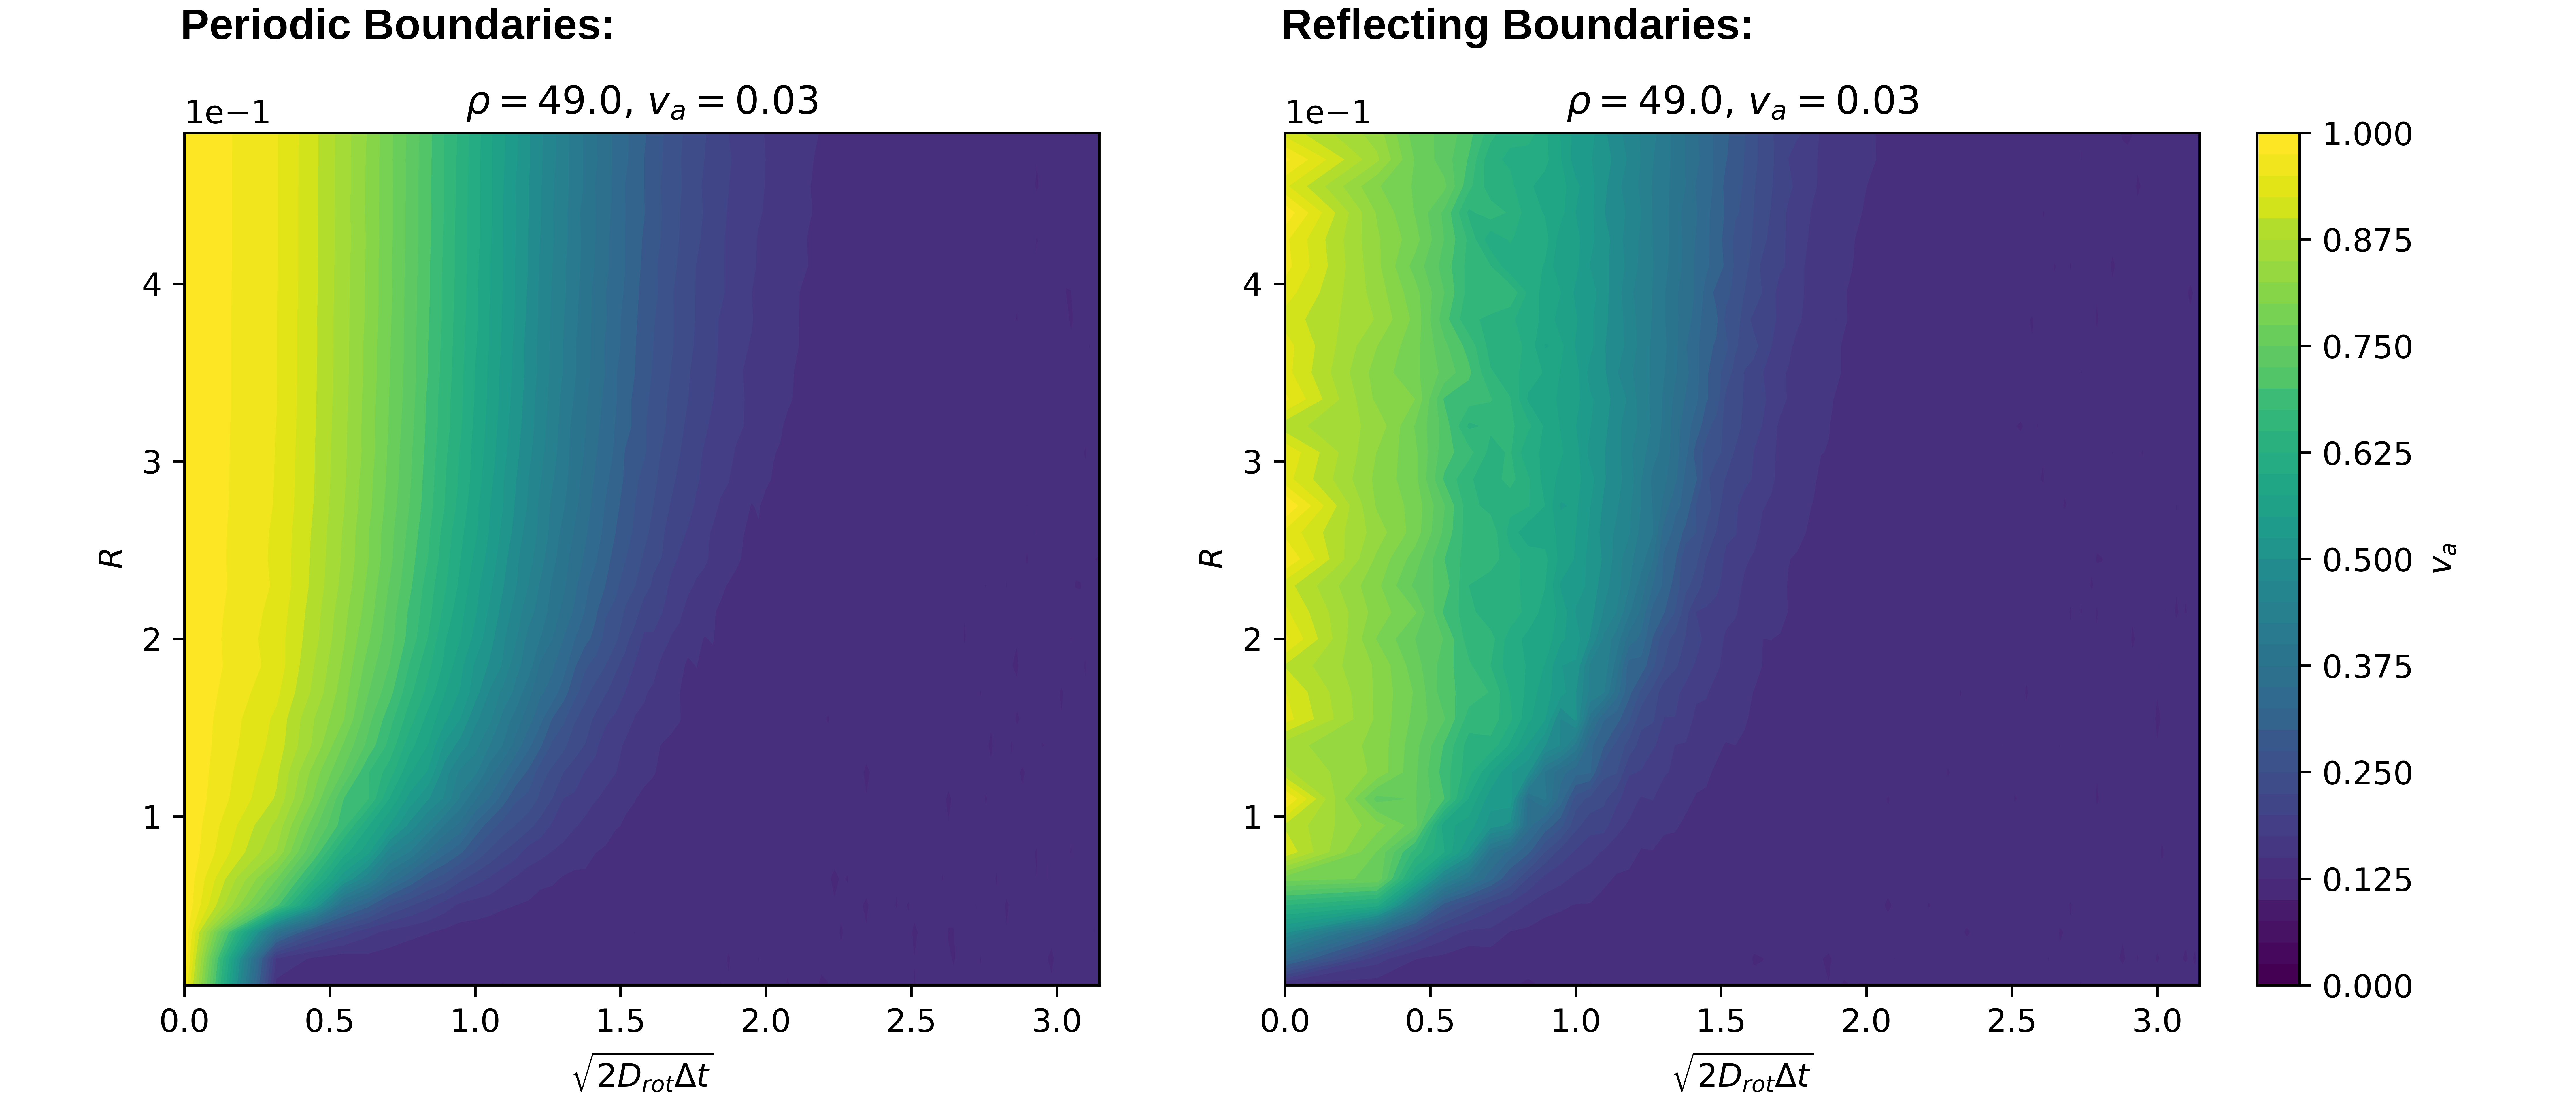
\includegraphics[width=0.9\textwidth]{images/chapter3/r_eta_transition_2D_comparison_pbc_rbc.png} 
  		%\caption*{Cantillano C., Grundpraktikum 2: Halbleiterbauelemente. Internal Proceedings. University of Innsbruck , 2021.}
	\end{figure}
\end{frame}

\begin{frame}
	\frametitle{3) Reflecting Boundaries}
	\textbf{Phase transitions.} 2D Levels in parameter space.
	\begin{itemize}
	    \item $\rho$ against $\sqrt{2D_{\text{rot}}\Delta t}$
	\end{itemize}
	\begin{figure}[H]
  		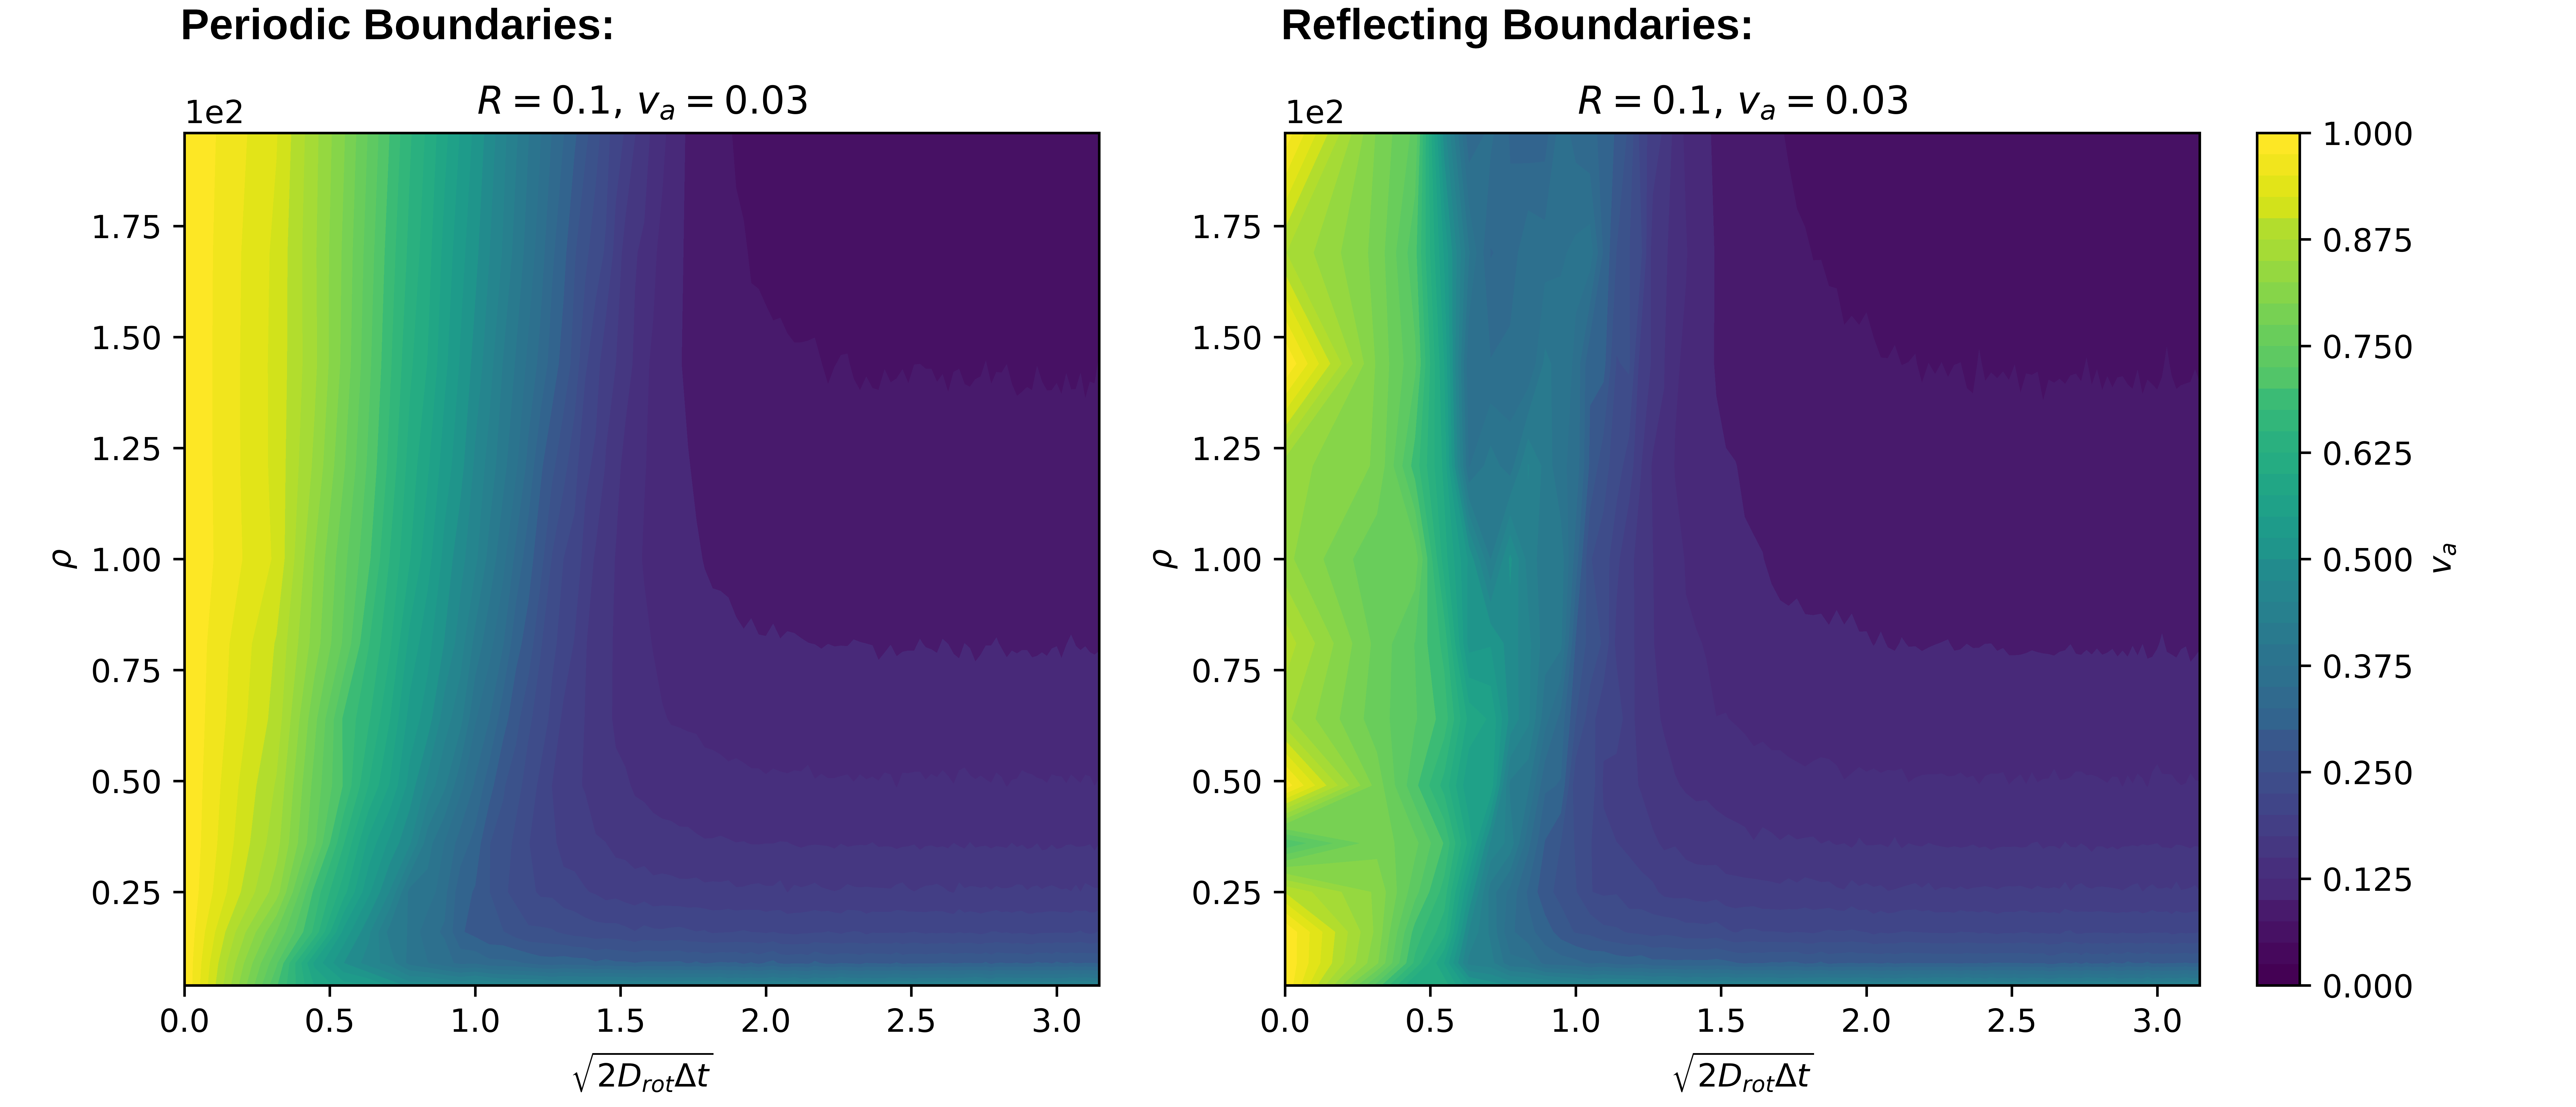
\includegraphics[width=0.9\textwidth]{images/chapter3/rho_eta_transition_2D_comparison_pbc_rbc.png} 
  		%\caption*{Cantillano C., Grundpraktikum 2: Halbleiterbauelemente. Internal Proceedings. University of Innsbruck , 2021.}
	\end{figure}
\end{frame}